\ifimagenes
\section{Marco teórico}
\else
\section{Reconstrucción del entorno}
\fi
\label{sec:marcoteorico}
En esta sección se presentan distintos métodos para poder realizar una reconstrucción del entorno en base a las nubes de puntos, además de dar una introducción a la librería de nube de puntos (PCL) y su vínculo con ROS, utilizados para el desarrollo del trabajo.

\ifimagenes
\subsection{Reconstrucción del entorno}
\else
\fi
En base a los datos provistos por los sensores exteroceptivos (LIDAR, cámaras, entre otros), el objetivo principal del trabajo consiste en recolectar dicha información para poder reconstruir el entorno en el cual se encuentra sumergido el robot, además de poder estimar su posición. Sin embargo, estos tipos de sensores proveen un campo de visión limitado, por lo que no es posible describir el mundo real como un todo en base a una sola medición de estos sensores, sino que solo puede mencionarse a una pequeña porción del mismo, denominada \textit{escena}.

A su vez, el tipo de dato que se tome de la escena dependerá del tipo de sensor extereoceptivo que los provea. Por ejemplo, una cámara monocular es capaz de otorgar imágenes 2D, mientras que con una cámara estéreo se consigue una nube de puntos 
\ifimagenes
    \ifimagenespaper
tridimensional.
    \else
tridimensional, tal como se describe en el apéndice.
    \fi
\fi

\subsection{Point cloud}
Una \textit{nube de puntos}, o de su terminología en inglés, \textit{point cloud}, se utiliza para describir a un conjunto de puntos de datos en un espacio dado. Las nubes de puntos 3D, por ejemplo, se tratan de un conjunto de puntos tridimensionales que se caracterizan por tener principalmente coordenadas espaciales XYZ, y opcionalmente pueden dar información de intensidad, color, entre otras.

Como se mencionaba anteriormente, la nube de puntos de la escena adquirida dependerá del principio de medición del sensor utilizado. En concreto, puede categorizarse en: \cite{weinmann2016}
\begin{itemize}
    \item \textit{Técnicas pasivas}, donde la luz ambiental se encuentra presente, permitiendo utilizar sensores como cámaras estéreo para obtener las imágenes propias del entorno.
    \item \textit{Técnicas activas} donde los sensores emiten radiaciones electromagnéticas, tal como es el caso de los LIDAR 3D o las cámaras infrarrojas.
\end{itemize}

Dependiendo de la técnica de adquisición involucrada y el dispositivo utilizado, los datos de la nube de puntos adquiridos pueden corromperse con más o menos ruido y, además de la información espacial en forma de coordenadas XYZ, los atributos de los puntos respectivos, como la información de color o intensidad también puede adquirirse, como se mencionaba anteriormente.

\subsection{Point Cloud Library (PCL)}
La \textit{Point Cloud Library (PCL)} se trata de un proyecto abierto desarrollado en \textit{C++} que ofrece herramientas para procesar imágenes o nubes de puntos tanto 2D como 3D. El framework PCL contiene numerosos algoritmos que realizan filtrado, estimación de características, reconstrucción de superficies, registro, ajuste de modelos y segmentación. Con estos métodos, es posible procesar la nube de puntos, extraer keypoints para reconocer objetos en el mundo en función de su apariencia geométrica, crear superficies a partir de las nubes de puntos y visualizarlas.

En general, PCL contiene una estructura de datos muy importante, que es $pcl::PointCloud$. Esta estructura de datos está diseñada como una clase de template que toma el tipo de punto que se utilizará como parámetro. Como resultado de esto, la clase de nube de puntos no es mucho más que un contenedor de puntos que incluye toda la información común requerida por todas las nubes de puntos independientemente de su tipo de punto. Algunos de los tipos de puntos más utilizados son
\begin{itemize}
    \item $pcl::PointXYZ$, el cual es el más simple que posee la librería, almacenando la información en XYZ únicamente
    \item $pcl::PointXYZRGB$, almacena además de la posición XYZ, el color en formato RGB de cada punto.
    \item $pcl::PointNormal$, representa la superficie normal en un punto dado y la medida de su curvatura, además de las coordenadas XYZ.
    \item $pcl::PointXYZI$, que a las coordenadas XYZ les asocia también información de intensidad del punto.
\end{itemize}

Debido al gran número de tipos de puntos que existen en la librería, cada algoritmo implementado en la misma refiere a una clase perteneciente a una jerarquía de clases con puntos en común específicos. Gracias a ello, dichos algoritmos pueden ser parametrizados en base a lo que necesite el usuario. 

\ifimagenes
    \ifimagenespaper
    \else
    \subparagraph{Interfaz con ROS}
    \fi
\fi
La interfaz PCL para ROS proporciona los medios necesarios para comunicar las estructuras de datos PCL a través del sistema de comunicación basado en mensajes proporcionado por ROS. Para hacerlo, hay varios tipos de mensajes definidos para contener nubes de puntos, así como otros productos de datos de los algoritmos PCL. En combinación con estos tipos de mensajes, también se proporciona un conjunto de funciones de conversión para convertir de tipos de datos PCL nativos en mensajes. Uno de los más importantes tipos de mensajes de ROS es el $sensor_msgs::PointCloud2$, el cual contiene una colección de puntos N-dimensionales, que pueden contener información adicional como normales, intensidad, entre otros.

Para relacionar ambos mundos, ROS cuenta con el paquete \textit{pcl\_conversions}\footnote{http://wiki.ros.org/pcl\_conversions}. Por ejemplo, en el Codigo \ref{lst:pc2pcl} se convierte un mensaje del tipo \lstinline{sensor_msgs::PointCloud2} a \lstinline{pcl::PointCloud<pcl::PointXYZRGB>}.

\begin{lstlisting}[caption=Conversión de mensaje ROS a PCL, label=lst:pc2pcl]
  // ROS PointCloud2
  sensor_msgs::PointCloud2 &pc2;
  
  // Output Cloud
  pcl::PointCloud<pcl::PointXYZRGB>::Ptr cloud_out(new pcl::PointCloud<pcl::PointXYZRGB>);
  // PCL PointCloud2
  pcl::PCLPointCloud2 pcl_pc2;   

  // Convert from ROS message to PCL data
  pcl_conversions::toPCL(pc2, pcl_pc2);
  pcl::fromPCLPointCloud2(pcl_pc2, *cloud_out);
\end{lstlisting}


\subsection{Adquisición de la nube de puntos}
Como se menciona en el documento, dependiendo del sensor utilizado para obtener los datos, se conseguirán las nubes de puntos asociadas dependiendo del principio de 
\ifimagenes
medición. A continuación se menciona en primera instancia una librería usada comúnmente en este tipo de aplicaciones (OpenCV), además de los sensores utilizados generalmente en este tipo de aplicaciones.

\subsubsection{OpenCV}
OpenCV\footnote{http://opencv.org} es una librería open source multiplataforma que busca brindar una infraestructura de visión artificial fácil de usar y que pueda utilizarse para aplicaciones de tiempo real, por lo que hace hincapié en la optimización. Para ello, OpenCV cuenta con un set de más de 500 funciones \cite{kaehler2017} que abarcan muchas áreas en visión, tales como calibración de cámaras, visión estéreo y robótica.

\subsubsection{Cámara estéreo}
Con el fin de poder simular el efecto de la percepción humana, las cámaras estéreo se ubican separadas una distancia fija y, por lo general, alineadas horizontalmente, como se observa la Bumblebee 2 en la Figura \ref{fig:stereoandrgbdcameras}.a. Al tener dos fuentes de imágenes distintas y ubicadas en una posición relativa conocida, es posible a partir de las mismas determinar la profundidad en la que se encuentran los objetos que ven entre ambas. 

Si bien se puede realizar con una cámara monocular, la técnica cuenta con mayor complejidad y con ciertas restricciones\footnote{Por ejemplo, sería necesario conocer una cierta cantidad de puntos claves del objeto para que, estando el mismo en una pose distinta a la analizada a priori, sea posible determinar la pose del objeto mediante estos puntos claves.}, aunque puede solventarse mediante el agregado de sensores que utilicen otro principio de medición\footnote{Las cámaras RGB-D, por ejemplo, cuentan con una cámara y sensores de distancia para determinar la ubicación de determinados píxeles.}.

Para poder conseguir una nube de puntos mediante el uso de dos cámaras, deben seguirse una serie de pasos \cite{kaehler2017}
\begin{enumerate}
    \item \textit{Remover las distorsiones} de la lente.
    \item Ajustar las distancias y ángulos entre las cámaras, conocido como \textit{rectificación}.
    \item Encontrar las mismas características en ambas cámaras, proceso conocido como \textit{correspondencia}. A partir de este se consigue un \textit{mapa de disparidad} (o \textit{disparity map}), donde las disparidades son las diferencias en la coordenada x de los planos de la imagen de la misma característica vista en las cámaras izquierda y dercha.
    \item Si se conoce el arreglo geométrico de las cámaras, puede cambiarse el mapa de disparidad en distancias por \textit{triangulación}. Este paso es denominado \textit{proyección}, y el resultado es un mapa de profundidad.
\end{enumerate}

Para obtener mejores resultados, es necesario que las cámaras estén sincronizadas entre sí, caso contrario los objetos en movimiento serán un problema.

\begin{figure}
    \centering
    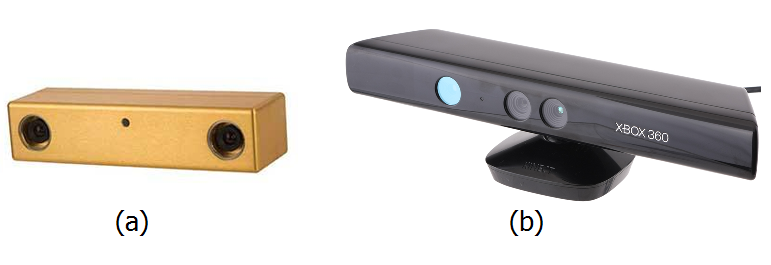
\includegraphics[width=.9\linewidth]{Img/bumblekinect}
    \caption{Cámaras: (a) Bumblebee 2, (b) Microsoft Kinect}
    \label{fig:stereoandrgbdcameras}
\end{figure}

\paragraph{Calibración}
La calibración estéreo depende de hallar la matriz de rotación y la traslación entre las dos cámaras previamente calibradas \cite{kaehler2017}, lo que puede realizarse mediante la función de OpenCV \texttt{cv::stereoCalibrate()}. En el mismo, se busca una sola matriz de rotación y un vector de traslación que relacione la cámara derecha con la cámara izquierda

Para la calibración en ROS se puede utilizar, al igual que en cámaras monoculares, el paquete \texttt{camera\_calibration}, el cual en este caso recibirá parámetros distintos. La interfaz gráfica para la calibración será similar al de cámaras monoculares, con la diferencia que en este caso aparecen ambas cámaras, aunque el principio de calibración del lado usuario es prácticamente el mismo, teniendo en cuenta que ahora en ambas cámaras debe visualizarse el patrón buscado, tal como se observa en la Figura \ref{fig:stereocalibrationchessboardrosexample}.
\begin{figure}
    \centering
    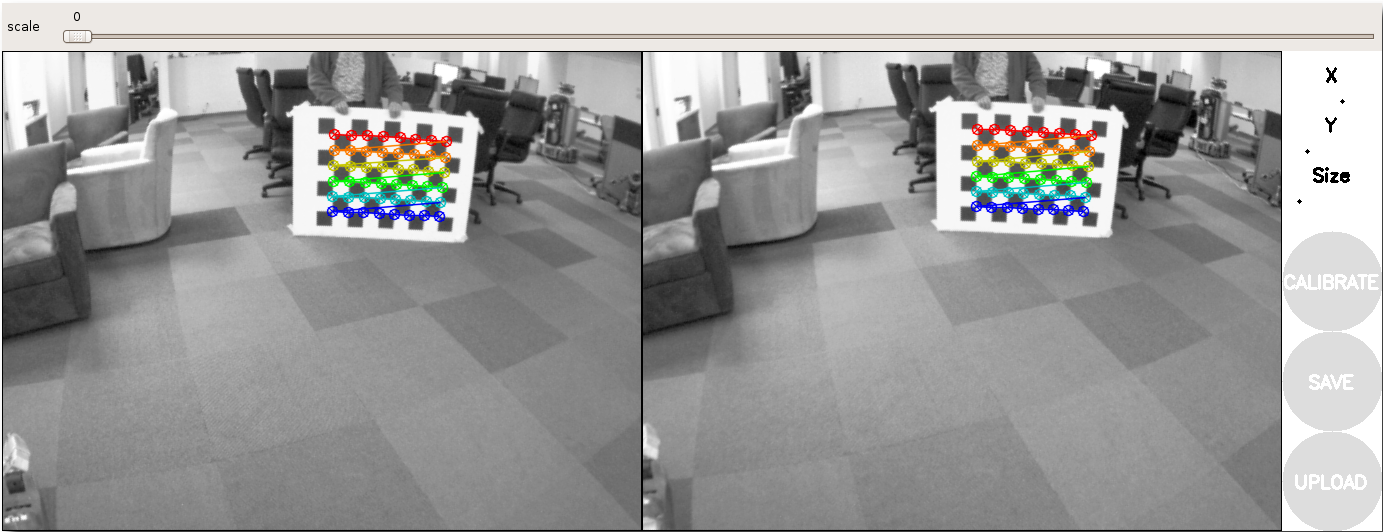
\includegraphics[width=\linewidth]{Img/StereoCalibrationChessboard.png}
    \caption{Calibración estéreo mediante ROS}
    \label{fig:stereocalibrationchessboardrosexample}
\end{figure}


\paragraph{Rectificación estéreo}
Si los planos de ambas cámaras no se encuentran perfectamente alineados, la disparidad estéreo aumenta su complejidad. Para poder mitigar este problema, lo que se busca es reproyectar los planos de la imagen de ambas cámaras para que residan en el mismo plano, conocido como \textit{rectificación estéreo}. Dentro de OpenCV, existen numerosas formas de obtenerlo, como pueden ser los algoritmos de Hartley o de Bouguet. El algoritmo de Hartley permite evitar la calibración de la cámara, en cambio para el segundo es necesaria.

Una vez que se obtienen los términos de la calibración estéreo, se pueden calcular los mapas de rectificación izquierda y derecha por separado utilizando para cada uno \texttt{cv::initUndistortRectifyMap()}.

En ROS, el paquete utilizado para dicha tarea es el denominado \texttt{stereo\_image\_proc}\footnote{\url{http://wiki.ros.org/stereo_image_proc}}, que permite obtener un mapa de profundidades. 

\paragraph{Correspondencia estéreo}
La correspondencia estéreo, esto es, coincidir un punto tridimensional en las vistas de ambas cámaras, requiere que estos puntos de ambas cámaras se solapen. Para ello, OpenCV implementa dos algoritmos distintos para correspondencias, convirtiendo dos imágenes (izquierda y derecha) en una sola imagen de profundidad
\begin{itemize}
    \item \textit{Block matching (BM) algorithm}, implementada mediante \texttt{cv::StereoBM()}, el cual es rápido y efectivo, aunque en escenas de baja textura presenta problemas. 
    \item \textit{Semi-global block matching (SGBM)}, implementada mediante \texttt{cv::StereoSGBM()}, el cual presenta una mayor exactitud que el BM, pero es computacionalmente más demandante.
\end{itemize}

En base a este proceso es que puede obtenerse una \textbf{nube de puntos} del entorno.

Para el caso de ROS, dentro del paquete \texttt{stereo\_image\_proc} se encuentra el ejecutable \texttt{dynamic\_reconfigure}\footnote{\url{http://wiki.ros.org/stereo_image_proc/Tutorials/ChoosingGoodStereoParameters}}, que permite modificar dinámicamente los parámetros de correspondencia, además de elegir el algoritmo a utilizar mediante una interfaz gráfica.

\subsubsection{Cámara RGB-D}
Las cámaras RGB-D\cite{hogman2011} en lugar de poseer dos cámaras monoculares presentan una cámara monocular con la ayuda de sensores infrarrojos para determinar la ubicación de determinados píxeles, siendo un ejemplo conocido de las mismas es la Microsoft Kinect, la cual se observa en la Figura \ref{fig:stereoandrgbdcameras}.b. Para que el mismo pueda obtener la nube de puntos, primero el sensor de distancia proyecta un patrón de moteado infrarrojo. El patrón proyectado es luego capturado por una cámara de infrarrojos en el sensor y comparado parte por parte con patrones de referencia almacenados en el dispositivo. Estos patrones fueron capturados previamente a profundidades conocidas en el proceso de calibración de los mismos. A continuación, el sensor estima la profundidad por píxel en función de los patrones de referencia con los que el patrón proyectado coincide mejor. Los datos de profundidad proporcionados por el sensor de infrarrojos se correlacionan luego con una cámara RGB calibrada. Esto produce una imagen RGB con una profundidad asociada a cada píxel. Una representación unificada popular de estos datos es una nube de puntos: una colección de puntos en un espacio tridimensional, donde cada punto puede tener características adicionales asociadas. Con un sensor RGB-D, el color puede ser una de esas características. Además, las normales de superficie aproximadas también se almacenan a menudo con cada punto en la nube de puntos resultante.
\else
medición, tal como se desarrolló en la Sección \ref{sec:sensors}.
\fi
\subsection{Point cloud registration}
Si bien un primer paso es obtener la nube de puntos en base al sensor utilizado, uno de los principales enfoques utilizados en robots móviles con los mismos es el llamado \textit{registro de nube de puntos} o, de su terminología en inglés, \textit{point cloud registration}. Dicho proceso responde a encontrar una transformación espacial que alinee dos nubes de puntos generalmente contiguas en el tiempo. Los sensores que utilizan normalmente este enfoque son las cámaras estéreo y RGB-D.

En concreto, dada una nube de puntos fuente (tambíen llamada \textit{input} o \textit{source}) $P$ con puntos $p \in P$, y una nube de puntos objetivo $Q$ (llamada \textit{target}) con puntos $q \in Q$, el problema del registro se basa en encontrar correspondencias entre $P$ y $Q$, y estimar una transformación $T$ que, cuando se aplica a $P$, se alinea todos los pares de puntos correspondientes ($p_i \in P$, $q_j \in Q$). Un problema fundamental del registro es que estas correspondencias generalmente no se conocen y deben ser determinadas por el algoritmo de registro. Dadas las correspondencias correctas, hay diferentes formas de calcular la transformación óptima con respecto a la métrica de error utilizada, como se detalla a continuación.

El registro de dos nubes de puntos puede dividirse en una serie de pasos, los cuales se observan en la Figura \ref{fig:registrationpipeline} y conforman el denominado \textit{registration pipeline}. El mismo si bien puede extenderse para un caso más general \cite{garcia2017}, en este caso se da una estructura representativa del trabajo presente, siendo dichos pasos la \textit{selección}, \textit{matcheo}, \textit{rejection} y \textit{alineación}.

\begin{figure}[!ht]
    \centering
    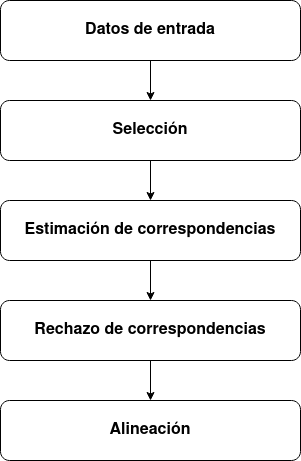
\includegraphics[width=0.45\linewidth]{Img/3DRegistrationPipeline.png}
    \caption{Registration pipeline}
    \label{fig:registrationpipeline}
\end{figure}

En primera instancia, debido a la gran densidad de puntos que presentan las nubes de puntos, además del ruido inherente de los sensores utilizados, es necesario realizar un proceso de \textit{selección} de los datos de interés, no solo para que el \textit{proceso de registro} pueda converger al valor óptimo, sino también para reducir el tiempo que tarda el algoritmo en completar el procesamiento.

Una vez que se tienen los datos seleccionados de cada una de las nubes de puntos a alinear, es necesario encontrar las correspondencias entre las mismas, esto es, encontrar un conjunto de puntos (los cuales suelen ser los \textit{keypoints}) en la nube de puntos fuente que se pueden \textit{identificar como los mismos puntos} en la nube de puntos objetivo.

En el proceso descripto anteriormente, normalmente una gran proporción de las correspondencias consideradas como tales en realidad son desajustes debidos al cambio de punto de vista, oclusión \cite{barazzetti2018}, entre otros. Estos desajustes suelen ser suficientes para arruinar los métodos de estimación tradicionales. Por lo tanto, es necesario eliminar o reducir la influencia indebida de los desajustes. Por ello, luego del pareo de los puntos característicos es necesario \textit{rechazar} las correspondencias para reducir el número de valores atípicos.

Finalmente, con las correspondencias filtradas, se busca la transformación que se ajusta mejor a ambas nubes de puntos mediante un proceso conocido como \textit{alineación}.

% \ifimagenes
% \else
% %% VA O NO VA?????
% A partir de la clasificación anterior, pueden diferenciarse dos tipos de algoritmos de registro, el \textit{registro basado en características (features)}, y los \textit{algoritmos de registro iterativos}, que se observan en la Figura \ref{fig:registrationprocess} y se detallan a continuación.
% \begin{itemize}
%     \item \textit{Registro basado en características (features)}, para calcular alineaciones iniciales, y
%     \item \textit{Algoritmos de registro iterativos}, siguiendo el principio del algoritmo ICP para iterativamente registrar nube de puntos (que ya se encuentran relativamente alineadas).
% \end{itemize}

% \begin{figure}[!ht]
%     \centering
%     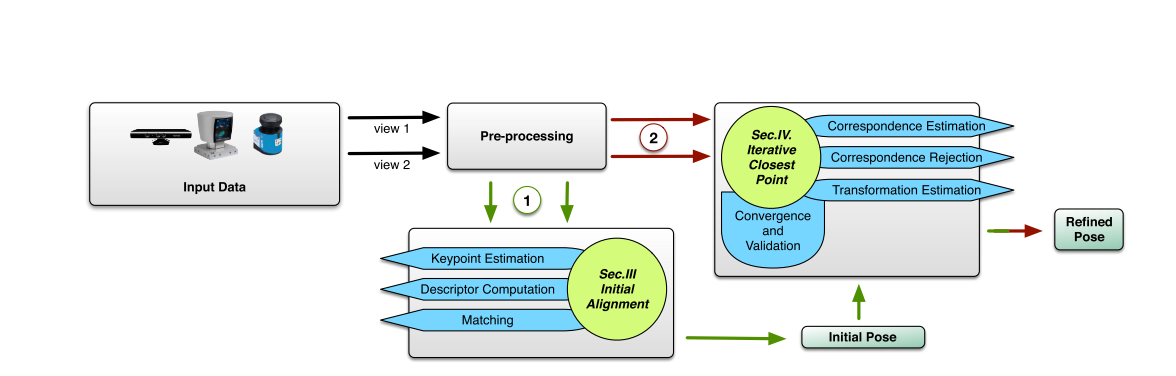
\includegraphics[width=\linewidth]{Img/RegistrationProcess.png}
%     \caption{Registration process}
%     \label{fig:registrationprocess}
% \end{figure}

% Para el registro basado en características, los descriptores de características geométricas se calculan y combinan en algún espacio de alta dimensión. Cuanto más descriptivos, únicos y persistentes sean estos descriptores, mayor será la probabilidad de que todas las \textit{coincidencias} (o \textit{correspondencias}) encontradas sean pares de puntos que realmente se correspondan entre sí.

% En el algoritmo ICP de Besl y McKay \cite{besl1992} no se calculan descriptores de características, sino que se considera que los puntos más cercanos en el espacio cartesiano se corresponden entre sí. Se estima una transformación que minimiza las distancias euclidianas entre pares encontrados de puntos más cercanos en el sentido de mínimos cuadrados. El proceso de determinar los puntos correspondientes en los dos conjuntos de datos y calcular la transformación que los alinea se repite iterativamente. Se espera que el conjunto de puntos de origen converja hacia el conjunto de destino a medida que las correspondencias sean cada vez mejores. Simultáneamente, Chen y Medioni \cite{chen1992} formularon un algoritmo similar, pero en lugar de minimizar las distancias euclidianas al cuadrado entre los puntos correspondientes, aplicaron una métrica de error de punto a plano.
% %%%%%
% \fi
A continuación, se desarrollan los pasos nombrados anteriormente.

\subsubsection{Selección}
Como la información suele ser redundate y lo suficientemente densa como para necesitar un gran costo computacional a la hora de procesar los datos, es necesario filtrar las nubes de puntos quitando la información irrelevante, reduciendo así el tiempo de ejecución de los algoritmos. Si bien existen en la literatura muchos criterios para decidir cuales puntos tomar y cuales no, en principio se pueden distinguir dos métodos de reducción de datos, siendo el primero el de extraer automáticamente un pequeño conjunto de keypoints únicos y repetibles, mientras que el otro se basa en muestrear los datos originales con respecto a una distribución objetivo deseada. Mientras que el primero está destinado a la alineación inicial basada en características \cite{merino2016}, el segundo se puede utilizar para reducir de manera eficiente la cantidad de datos para los algoritmos de registro iterativos. PCL implementa varios de estos métodos de muestreo, en particular, el muestreo en el espacio índice (simplemente tomando cada n-ésimo punto), submuestreo uniforme en el espacio 3D de entrada (para capturar mejor las estructuras ambientales detectadas) y muestreo en el espacio de normales de superficie (para muestrear puntos en todas las orientaciones de la superficie). A continuación se presentan dos métodos que suelen emplearse en este tipo de tareas
\begin{itemize}
    \item \textit{Normal space sampling}: Al tratar generalmente con modelos suaves con pequeñas irregularidades (por ejemplo, un plano), el proceso puede resultar en el muestreo de muchos puntos que contienen esencialmente la misma información en términos de vectores normales. Por ello, la estrategia de \textit{normal space sampling} pretende dar uso a esta información \cite{rusinkiewicz2001}, y la misma consiste en, en primera instancia, agrupar puntos en ''cubos'' de acuerdo con los ángulos entre sus vectores normales (considerados en la esfera unitaria) y los ejes de coordenadas, y luego muestrear uniformemente sobre los cubos resultantes, proporcionando un submuestreo de los puntos con más vectores normales "frecuentes". Dentro de PCL, este algoritmo se encuentra implementado en el método \lstinline{pcl::NormalSpaceSampling}.
    \item \textit{Harris 3D}: El operador de Harris \cite{harris1988} se trata de un detector de puntos de interés para imágenes. El método es una técnica popular debido a su fuerte invariancia a la rotación, escala, variación de iluminación, y ruido de imagen \cite{schmid2000}. El detector de Harris se basa en la función de autocorrelación local de una señal, que mide los cambios locales de la señal con parches desplazados una pequeña cantidad en diferentes direcciones. El mismo se ha utilizado en muchas aplicaciones en procesamiento de imágenes y visión artificial por su sencillez y eficiencia. Sin embargo, el problema con los datos 3D es que la topología es arbitraria y no está claro cómo calcular las derivadas. Para solucionar este problema, en \cite{sipiran2011} proponen transformar a los puntos de la nube de la siguiente manera
    \begin{enumerate}
        \item Por cada punto de la nube, se define un \textit{punto vecino} del mismo, y se calcula el centroide de este último
        \item Todos los puntos de la nube se trasladan para que el centroide coincida con el origen de coordenadas
        \item Luego, se calcula un plano de ajuste a los puntos traslada
        \item Se aplica el \textit{análisis de componentes principales} (PCA de sus siglas en inglés) \cite{jollife2016} al conjunto de puntos y se elige el \textit{eigenvector} con el \textit{eigenvalue} asociado más bajo como la normal del plano de ajuste.
        \item Se rotan los puntos hasta que la normal al plano coincide con el eje z.
        \item El plano XY resultante se utiliza para calcular las derivadas. Estas derivadas se calculan utilizando una superficie cuadrática de seis términos (paraboloide) ajustada al conjunto de puntos transformados.
    \end{enumerate}
    Dentro de PCL, en el método \lstinline{pcl::HarrisKeypoint3D} se encuentra una implementación de dicho algoritmo.
\end{itemize}

\subsubsection{Estimación}
La estimación de correspondencias es el proceso de emparejar los puntos $p_i$ desde la nube de puntos fuente $P$ con sus vecinos más cercanos $q_j$ en la nube objetivo $Q$. 

En PCL, con la función \lstinline{pcl::registration::DetermineCorrespondences} se obtiene el conjunto de pares de correspondencia encontrados entre el la nubes de puntos fuente y objetivo. Cada par consta del índice del punto en la nube de origen y el índice de la coincidencia encontrada en la nube de puntos de destino. 

En el caso de datos de entrada provenientes de sensores que cumplen con el modelo de cámara estenopeica \cite{kaehler2017}, el procedimiento de estimación de correspondencia puede acelerarse significativamente con la contraparte de perder algo de precisión. Estos sensores incluyen cámaras RGB-D populares como Microsoft Kinect, y recopilan información del entorno en forma de imágenes de profundidad y color. En árboles PCL para búsquedas de vecinos más cercanos en el espacio 3D, es posible utilizar la naturaleza proyectiva de las imágenes de profundidad para obtener una aproximación razonable. Cada punto de la nube corresponde a un píxel en la imagen de profundidad, lo que permite proyecciones desde puntos de origen en coordenadas mundiales hasta el plano de la cámara del marco de destino mediante el uso de parámetros de cámara intrínsecos y extrínsecos. Este enfoque es rápido, pero impreciso para nubes de puntos con grandes discontinuidades de profundidad o para cuadros que están muy alejados entre sí. Es por eso que se recomienda usar este método solo después de que las dos nubes de puntos se hayan acercado, lo que lo hace bueno para alinear nubes de puntos consecutivas en una secuencia grabada a alta velocidad de cuadros.

%% QUE ONDA CON ESTO???
% Los métodos que extraen pocos keypoints pueden utilizar la fuerza bruta para encontrar correspondencias. Sin embargo, este proceso es computacionalmente costoso. Algunos métodos reducen el tiempo de cálculo minimizando el espacio de búsqueda, como 3D Shape Context [69] que preselecciona los posibles candidatos que satisfacen ciertos criterios y luego aplica fuerza bruta con estos candidatos. No obstante, en la mayoría de las situaciones, se necesitan algoritmos más elaborados para informar los resultados en un período de tiempo razonable.

% Como se necesitan al menos tres puntos no coplanares en cada conjunto para determinar una transformación rígida entre dos conjuntos de puntos 3D sin ambigüedad, el costo asintótico de tales enfoques está en O (n6). En consecuencia, el espacio para navegar en la búsqueda de correspondencias es enorme. Diseñar una estrategia de búsqueda sofisticada que sea capaz de aprovechar la información de detección y descripción tiene el potencial de reducir en gran medida los costos de cálculo y, por lo tanto, aumentar el rango de aplicación de tales algoritmos de registro. Los métodos existentes que implementan estrategias de búsqueda ya logran muy buenos resultados en comparación con los métodos típicos de fuerza bruta.

% A diferencia de los algoritmos de alineación, la finalidad de estas estrategias de coincidencia es lograr solo una alineación aproximada. La idea es identificar la posición arbitraria de las formas de entrada y encontrar las transformaciones entre ellas, lo más rápido posible. La precisión no es, por tanto, el factor más importante. En cambio, la robustez es clave proporcionando garantías para el posterior ajuste fino.
% A continuación se presentan algunos métodos conocidos de la literatura.

% \paragraph{Métodos basados en RANSAC}
% RANdom SAmple and Consesus (RANSAC) es un método iterativo diseñado para encontrar los parámetros de un modelo a partir de un conjunto de datos que contiene valores atípicos (\textit{outliers}). Dada una entrada de datos ruidosos, RANSAC encuentra los parámetros que ajustan los datos de entrada a un modelo dado, descartando los valores atípicos. Este enfoque es la base de una amplia variedad de métodos. Uno de ellos es el enfoque presentado por [34] que se basa en el hecho de que podemos determinar una transformación rígida con solo tres puntos (una base B). La idea es encontrar una base en una de las formas y encontrar la base correspondiente en la otra forma. El algoritmo funciona de la siguiente manera: 
% \begin{itemize}
%     \item primero, determina tres puntos diferentes al azar en la primera superficie: primario (ap), secundario (as) y auxiliar (aa). Considere que las distancias entre estos tres puntos son dps, dpa y dsa. Cada punto en la segunda superficie se considera como el punto correspondiente bp del punto primario ap en la primera superficie.
%     \item Luego, se busca la correspondencia del punto secundario en la segunda superficie a una distancia dps de bp. Si no existe ningún punto alrededor de bp a la distancia dps, descarte bp y comience de nuevo con otro punto primario en la segunda superficie. Sin embargo, si hay un punto secundario bs busque el punto auxiliar ba que satisface las distancias. La transformación entre ambas superficies se puede determinar cuando se identifica la base BB en la segunda superficie. Esta búsqueda se repite para todas las bases encontradas. La mejor transformación es la que tiene el mayor número de puntos correspondientes.
% \end{itemize}

% Aunque este método es robusto incluso con valores atípicos, el principal inconveniente es su tiempo de cálculo. De hecho, este método solo se puede utilizar con una pequeña cantidad de datos de entrada.

% Dentro de PCL, el método \lstinline{pcl::RandomSampleConsensus} representa una implementación del algoritmo RANSAC, tal como se describe en \textbf{[Fischler,1981]}.

% \paragraph{}
%%

%% VER SI PONER O QUE HACER







% \subsubsection{Decimación y filtrado}
% Uno de los grandes problemas que presentan las nubes de puntos al querer hacer un procesamiento de las mismas refieren a la gran densidad de puntos y al\usepackage{comment} ruido en si. Para el primer caso, por ejemplo, si se tiene una nube de 640x480 (estándar), se tendrían que procesar entonces 307200 puntos, generando que se requiera mucho tiempo para completar el procesamiento del algoritmo. El segundo problema, en cambio, genera que se malinterprete la información, provocando resultados incorrectos. 

\subsubsection{Rechazo}
Dado que las correspondencias no válidas pueden afectar negativamente los resultados del registro, la mayoría de los procesos de registro presentan un paso de rechazo. El mismo consiste en filtrar los pares de puntos emparejados en la etapa anterior para facilitar el algoritmo de estimación de la transformación hacia la convergencia al mínimo global. Este paso puede aprovechar la información auxiliar disponible de las nubes de puntos de entrada, como las normales de superficie locales o las estadísticas sobre las correspondencias. A continuación se detallan algunos de los algoritmos más utilizados
\begin{itemize}
    \item \textit{Rechazo de correspondencias basado en la distancia}: en base a un umbral, se filtran las correspondencias que estén a una distancia mayor que dicho límite. En PCL, se implementa mediante \lstinline{pcl::registration::CorrespondenceRejectorDistance}.
    \item \textit{Rechazo en base a la distancia mediana}: a diferencia del método anterior, en este caso el umbral se calcula en base a la mediana de todas las distancias punto a punto en las correspondencias estimadas inicialmente. Se utiliza la mediana ya que suele ser más efectiva en reducir la influencia de valores atípicos. El método \lstinline{pcl::registration::CorrespondenceRejectorMedianDistance} implementa dicha operación.
    \item \textit{Rechazo basado en RANSAC}: Este método aplica el RANdom SAmple Consensus \cite{fischler1981} para estimar una transformación para subconjuntos del conjunto dado de correspondencias y elimina las correspondencias atípicas basadas en la distancia euclidiana entre los puntos después de que la transformación calculada se aplica a la nube de puntos fuente. Es muy eficaz para evitar que el algoritmo ICP converja en mínimos locales, ya que siempre produce correspondencias ligeramente diferentes y es bueno para filtrar valores atípicos. Además, proporciona buenos parámetros iniciales para la estimación de la transformación con todas las correspondencias internas que siguen. El mismo cuenta con el método de PCL \lstinline{pcl::registration::CorrespondenceRejectorSampleConsensus}.
    \item \textit{Rechazo basado en la compatibilidad normal}: este filtro usa la información normal sobre los puntos y rechaza aquellos pares que tienen normales inconsistentes, es decir, el ángulo entre sus normales es mayor que un umbral dado. Puede rechazar pares erróneos que parecen correctos cuando se juzgan solo por la distancia entre los puntos. El mismo es implementado por \lstinline{pcl::registration::CorrespondenceRejectorSurfaceNormal}.
\end{itemize}

\subsubsection{Alineación}
A lo largo de los años, ha habido numerosos enfoques matemáticos para resolver la transformación rígida $T$ que minimiza el error de los pares de puntos. $T$ se compone de una rotación $R$ y una traslación $t$. Tenga en cuenta que, a continuación, cuando se hace referencia a una transformada $T$ y un punto $p$, se utilizarán coordenadas homogéneas. Hay dos métricas de error principales que se deben minimizar y que se han considerado en la literatura: \textit{punto a punto} (Ec. 2) y \textit{punto a plano} (Ec. 3), donde ($p_k$, $q_k$) es el \textit{k-ésimo} de el par $N$ corresponde desde la nube de origen a la nube de destino.
\begin{itemize}
    \item Métrica de error estándar de punto a punto: La métrica de error estándar utilizada en el algoritmo ICP es la métrica de error de punto a punto (Ec. 2). Fue mencionado por primera vez por Arun \cite{arun1987}; los investigadores propusieron varias formas de minimizarlo, seguidas de la introducción del algoritmo ICP \cite{besl1992}. Eggert y col. \cite{eggert1997} evaluó cada uno de estos métodos en términos de estabilidad numérica y precisión, llegando a la conclusión de que tienen un desempeño cercano. PCL ofrece una implementación (\lstinline{pcl::registration::TransformationEstimationSVD}) utilizando \textit{descomposición en valores singulares} (SVD), propuesto en primera instancia por \cite{horn1987}.
    \item \textit{Métrica de error de punto a plano}: Chen y Medioni \cite{chen1992} introdujeron la métrica de punto a plano (Ec. 3) y demostraron que es más estable y converge más rápido que los enfoques anteriores. Utiliza la distancia entre el punto de origen $\bm{p}_k$ y el plano descrito por el punto de destino $\bm{q}_k$ y su normal de superficie local $n_{\bm{q}_k}$. A diferencia de la métrica punto a punto, no tiene una solución de forma cerrada, por lo que la minimización se realiza con solucionadores no lineales (como Levenberg-Marquadt), o linealizándolo \cite{low2004} (bajo el supuesto de ángulos de rotación pequeños, es decir, $sin \theta \sim \theta$ y $cos \theta \sim 1$). Dependiendo de la superficie subyacente y la distribución de puntos, el uso de la métrica de error de punto a plano puede ser considerablemente más robusto. Un procedimiento estándar para minimizarlo se basa en el optimizador no lineal de Levenberg-Marquardt \cite{fitzgibbon2001}. Dicha funcionalidad se emplea en \lstinline{pcl::registration::TransformationEstimationPointToPlane}.
    \item \textit{Métrica de error punto-a-plano ponderada}: Asignar un peso diferente a cada correspondencia puede mejorar la convergencia. La ponderación de los pares de puntos puede verse como un rechazo de correspondencia suave, ajustando la influencia de los puntos correspondientes ruidosos en el proceso de minimización. La ponderación puede ser una función de la distancia punto a punto o punto a plano entre los puntos, una función del ángulo entre las normales correspondientes a los puntos, o una función del modelo de ruido del sensor que se ha usado. Un ejemplo de PCL puede ser \lstinline{pcl::registration::TransformationEstimationPointToPlaneWeighted}.
\end{itemize}

\subsection{Point Cloud 2D}
Si bien las nubes de puntos tridimensionales son una generalización de aquellas que refieren a dos dimensiones, el hecho de tener información sólo de un plano reduce drásticamente la cantidad de puntos a analizar. Este caso sucede en sensores como los LIDAR 2D, donde midiendo el tiempo de vuelo de la señal láser se logran conocer la distancia de distintos puntos de los objetos respecto al sensor. Es por esto que el enfoque de reconstrucción del entorno no suele ser el mismo que el descripto anteriormente.

\subsubsection{Algoritmo para LIDAR 2D}
Al igual que con el método descripto anteriormente, en la reconstrucción de mapas 2D se pretende conseguir la transformación que mejor responda al movimiento del robot entre el instante de tiempo actual y el anterior. Un algoritmo común de coincidencia de escaneo láser encuentra la transformación óptima de cuerpo rígido $T$ que alinea el escaneo láser actual $S_t$ en el tiempo $t$ con el anterior $S_{t-1}$ en el tiempo $t-1$. Este método solo considera dos escaneos láser secuenciales, y cuando se aplican iterativamente para todos los escaneos láser uno por uno, el problema de deriva de pose se deterioraría debido a los errores de coincidencia acumulados, lo que afectará la precisión de la siguiente coincidencia. 

Para abordar este inconveniente, en lugar de comparar los datos en el instante $t$ con el anterior, $t - 1$, se puede comparar dicha información actual con el mapa generado anteriormente, $M_{t-1}$, el cual es generado por todos los escaneos anteriores, de $1$ a $t-1$, y, en caso de ser un occupancy grid map, almacena el valor de probabilidad de cada celda de la cuadrícula en la región del espacio 2D. De acuerdo con las Reglas de Bayes, asumiendo la independencia de cada punto de $S_t$, el valor de probabilidad de la suma de $S_t$ respecto al mapa $M_{t-1}$ se calcula como
\begin{equation}
    p(S_t|M_{t-1}) = \sum_{x\epsilon S_t} p(x|M_{t-1})
\end{equation}
siendo $p(x|M_{t-1})$ la probabilidad de que un punto de escaneo $x \epsilon S_t$ coincida con uno perteneciente a $M_{t-1}$ en esa misma ubicación. Entonces, para buscar la transformación de $S_t$ que mejor se adapte al movimiento del robot respecto al mapa generado anteriormente $M_{t-1}$, llámese $T^*$, puede aplicarse el método de máxima verosimilitud
\begin{equation}
    T^* = argmax(p(T\propto S_t|M_{t-1})
\end{equation}
donde $T\propto S_t$ refiere a los datos del sensor en el instante actual $S_t$ transformados por $T$. A continuación, se presentan una serie de pasos a seguir para lograr el objetivo.

\paragraph{Filtrado de los datos}
Un ejemplo de los datos provenientes de un LIDAR 2D pueden verse en la Figura \ref{fig:lidar2dpoints}. Tal como en el caso de las nubes de puntos tridimensionales, para el caso del LIDAR 2D es necesario quedarse sólo con los datos de mayor relevancia. Por ejemplo, un punto en el espacio sin otros cercanos no aportará mucha información, mientras que una conglomeración de puntos puede resultar en una pared, por ejemplo.

\begin{figure}[!ht]
    \centering
    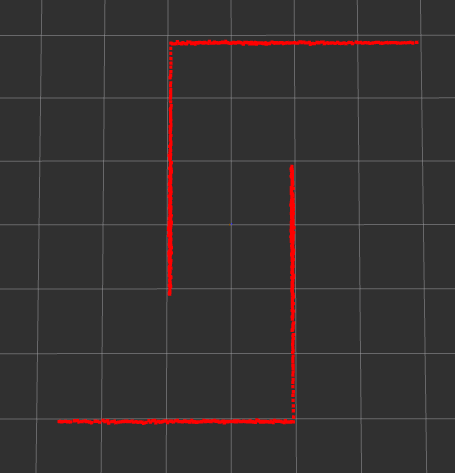
\includegraphics[width=0.75\linewidth]{Img/LIDAR2DPoints.png}
    \caption{Puntos dados por un LIDAR 2D}
    \label{fig:lidar2dpoints}
\end{figure}

Existen numerosas técnicas para obtener los distintos puntos de interés, ya sea filtrando en base a la distancia entre los puntos, como también la extracción de líneas en base a dichos puntos \textbf{(Gao, 2018)}.

\paragraph{Estimación de la transformación óptima}
En concreto, hay dos formas principales de encontrar la transformación de cuerpo rígido óptima: una es mediante métodos de búsqueda bruta y la otra es la que se basa en el ascenso en gradiente. El método de ascenso en gradiente puede atascarse en el mínimo local, mientras que el método de búsqueda bruta es una búsqueda global y es más robusto. Además, un mapa de múltiples resoluciones y una ventana de búsqueda estrecha pueden mejorar en gran medida la eficiencia de búsqueda del método de búsqueda bruta en una aplicación en tiempo real costosa en tiempo \textbf{(Olson, 2009)(Olson, 2015)}.

\subsubsection{Generación de mapas con LIDAR 2D}
Como los LIDAR en si no aportan información de colores, sino que para el caso de los bidimensionales la misma se trata de puntos en un plano, como se observa en la Figura \ref{fig:lidar2dpoints}, los mapas generados por dichos sensores suelen ser son los \textit{occupancy grid maps} vistos en la Sección \ref{sec:slam}, donde a partir de la ubicación de los puntos provistos por el sensor se determinan los lugares ocupados y libres, siendo las casillas libres las que se encuentran entre el sensor y cada punto y las ocupadas las correspondientes a la posición de los puntos en si, tal como se observa en la Figura \ref{fig:lidar2dmap}. Si bien existen los mapas binarios, en los que se tiene \textit{ocupado, vacio} o \textit{desconocido} solamente, al existir un margen de error en las mediciones, dichos mapas suelen ser probabilísticos, siendo 0.5 el valor por defecto de todas las celdas desconocidas.

\begin{figure}[!ht]
    \centering{{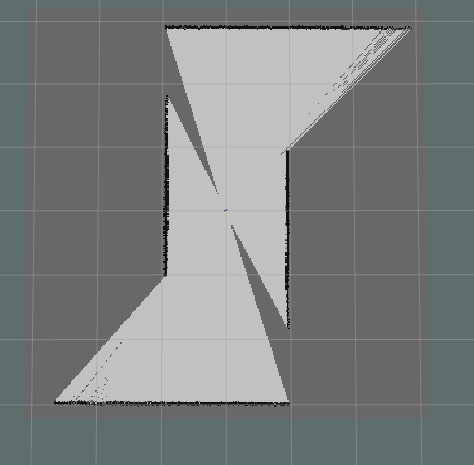
\includegraphics[width=0.75\textwidth]{Img/LIDAR2DMap.png}}}%
    \caption{Mapa generado a partir de los datos del LIDAR 2D}
    \label{fig:lidar2dmap}
\end{figure}

Para poder conseguir el mapa mencionado anteriormente, se tienen que seguir una serie de pasos y tener ciertas consideraciones, las cuales se desarrollan a continuación.

\paragraph{Obtención de las distintas celdas}
Como se trata de un mapa basado en grillas, se deben determinar no solo las celdas que se corresponden con cada punto, sino también aquellas que corresponden a las celdas libres entre los puntos y el sensor.

En el primer caso, al tener la resolución del mapa y la cantidad de cuadros en el mismo, pueden determinarse sin problemas las posiciones de los puntos dados por los datos del LIDAR. 

Para el segundo caso, en cambio, como se dispone a priori de la coordenada del punto y la ubicación del sensor, se podría trazar una recta entre dichos puntos. A partir de la misma, en base a la grilla utilizada, se necesita conocer cuáles celdas atraviesa dicha línea y cuáles no. Un método comúnmente utilizado en este tipo de problemas es el algoritmo de Bresenham \textbf{(Bresenham, 1965)}, permitiendo conseguir los resultados observados en la Figura \ref{fig:bresenhamlinealgorithm}.

\begin{figure}[!ht]
    \centering
    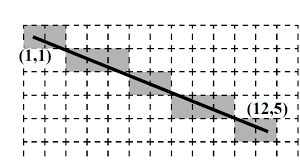
\includegraphics[width=0.9\linewidth]{Img/BresenhamLineAlgorithm.png}
    \caption{Ejemplo del algoritmo de Bresenham en base a una grilla dada. En negro se observa la línea de la cual se parte, y las celdas en gris son las que se obtienen a partir del algoritmo.}
    \label{fig:bresenhamlinealgorithm}
\end{figure}

\paragraph{Ponderación de las celdas}
Como se mencionaba anteriormente, los mapas suelen ser probabilísticos debido al ruido inherente de los sensores. Para poder determinar los valores que debe tomar cada celda (entre 0 y 1), suele ser recurrente el \textit{desenfoque Gaussiano} (del inglés \textit{Gaussian blur}), el cual se basa en desenfocar una imagen mediante una función Gaussiana. Si bien el mismo suele conocerse para una dimensión, puede extenderse a dos dimensiones sin mucho esfuerzo \textbf{(Haddad, 1991)}, ya que se trata del producto de dos Gaussianas, una en cada dimensión.

\paragraph{Actualización del mapa}
Una vez obtenido el mapa basado en la medición actual y, por ende, la transformación que describe el movimiento del robot, se procede a la actualización del mapa generado en los instantes de tiempo anteriores. Para poder realizar esto, una forma sería mediante la actualización de Bayes, vista en la Sección \ref{sec:regressionanalysis} y representada por la Expresión (\ref{eq:posteriorfull}). El problema de la misma es que, si se multiplican valores muy pequeños, el costo computacional aumenta. Una forma de mitigar este inconveniente es mediante el uso de la función \textit{logit}, la cual se basa en un número $p$ entre $0$ y $1$ que responde a la forma

\begin{equation}
    logit(p) = \log\left(\frac{p}{1-p}\right)
\end{equation}
obteniendo entonces valores entre $-\infty$ y $+\infty$, tal como se observa en la Figura .a. Para volver a la forma de probabilidad comúnmente utilizada, observada en la Figura .b, se utiliza la siguiente Expresión, la cual se consigue despejando la anterior
\begin{equation}
    p = \frac{e^{logit(p)}}{1+e^{logit(p)}}
\end{equation}

Partiendo entonces de la Expresión (\ref{eq:posteriorfull}), separando la medición actual de las anteriores y utilizando la suposición de Markov, la cual define que la medición actual es independiente de las mediciones anteriores si el estado actual es conocido, se llega a
\begin{equation}
    p(m_i|y_{1:t}) = \frac{p(y_t|m_i)p(m_i|y_{1:t-1})}{p(y_t|y_{1:t-1})}
\end{equation}
siendo 
\begin{itemize}
    \item $m_i$ la celda actual del mapa,
    \item $y_{1:t}$ las mediciones del sensor en esa celda desde el tiempo $1$ al tiempo $t$, 
    \item $p(y_t|m_i)$ la probabilidad de la medición actual dado el estado de la celda,
    \item $p(m_i|y_{1:t-1})$ la probabilidad de que una celda esté ocupada dadas todas las mediciones anteriores, y
    \item $p(y_t|y_{1:t-1})$ la probabilidad de tener una medición $y_t$ dadas todas las mediciones anteriores $y_{1:t-1}$.
\end{itemize}


Si se expande $p(y_t|m_i)$ mediante la regla de Bayes
\begin{equation}
    p(y_t|m_i) = \frac{p(m_i|y_t)p(y_t)}{p(m_i)}
\end{equation}
y se aplica a la Expresión anterior, se obtiene
\begin{equation}
    p(m_i|y_{1:t}) = \frac{p(m_i|y_t)p(y_t)p(m_i|y_{1:t-1})}{p(m_i)p(y_t|y_{1:t-1})}
\end{equation}

Luego, aplicando la fracción presente en la función \textit{logit}, se puede llegar a
\begin{equation}
    \frac{p(m_i|y_{1:t})}{1-p(m_i|y_{1:t})} = \frac{p(m_i|y_t)(1-p(m_i))p(m_i|y_{1:t-1})}{(1-p(m_i|y_t))p(m_i)(1-p(m_i|y_{1:t-1})}
\end{equation}

Finalmente, aplicando el logaritmo,
\begin{equation}
    logit(p(m_i|y_{1:t})) = logit(p(m_i|y_t)) + logit(p(m_i|y_{1:t-1})) - logit(p(m_i))
    \label{eq:logitupdatemap}
\end{equation}
resultando entonces la actualización del mapa en la adición de tres funciones \textit{logit}, siendo el primer término el referido al valor de la celda en base a la medición actual, el segundo correspondiente al valor de la celda respecto a las mediciones anteriores, y el tercero corresponde al valor de la celda en el instante inicial (siendo desconocido, $m_i = 0.5$ generalmente).

\subsection{Resumen}
En esta Sección, se presentó el concepto de nube de puntos, a su vez de mencionar las características de la \textit{Point Cloud Library} en este tipo de aplicaciones, siendo una herramienta esencial para el desarrollo del trabajo presentado.

A su vez, se presentaron los distintos métodos para la generación de mapas 2D, además de mencionar las técnicas utilizadas para la estimación del movimiento según los datos acutales y los anteriores.